\documentclass{article}

\usepackage{fullpage,amsmath,amsthm,amsfonts,amssymb,graphicx,enumitem}
\usepackage{algpseudocode}

\theoremstyle{definition}
\newtheorem{thm}{Theorem}
\newtheorem{question}[thm]{Question}
\newenvironment{answer}{\noindent\textit{Answer:}}{}

\title{Quiz 1 Practice Questions}
\author{ASEN 6519-001: Advanced Survey of Sequential Decision Making}

\begin{document}

\maketitle

\section{Questions from Papers}

\begin{question}
Why does ACAS Xu use an offline defined lookup table as part of the solution to providing guidance advisories? If a lookup table was not used and the entire problem was calculated online, what would be an adequate method of solving the application?
\end{question}

\begin{answer}
ACAS Xu uses an offline lookup table to reduce the complexity of generating real-time collision avoidance. Solving known and predictable portions of the problem ahead of time allows for more factors to be taken into account during flight. If a lookup table were not utilized, then an online solver such as POMCP/PO-UCT could provide adequate guidance, although it would not be as efficient in execution or reliably accurate as using the proposed ACAS Xu architecture.
\end{answer}

\begin{question}
If a MDP or POMDP could not be used to solve the ACAS Xu problem, how else might collision avoidance recommendations be provided? Why is this approach not utilized?
\end{question}

\begin{answer}
If MDPs cannot be used to solve the problem, collision avoidance recommendations could be defined by rule based decision making that cover all possible aircraft and intruder states. As every possible edge case must be defined, this quickly becomes intractable and results in unnecessary and inefficient collision avoidance recommendations.    
\end{answer}

\begin{question}
Convolutional Neural Networks (CNNs) are useful for object identification and feature detection. One of the basic uses of CNNs is for edge detection. In the NVIDIA paper on self-driving cars, the authors demonstrated that the final CNNs were able to clearly identify the road edges in the first few layers. Given a 4x4 matrix with 1’s and 0’s representing two different terrains, come up with the elements of a 2x2 convolution kernel which transforms the original matrix to a 3x3 with 1’s indicating the edge (separating original 1’s and 0’s). Note that the kernel has a 1x1 stride, and no padding (kernel does not go outside the original matrix bounds). Note that the convolution operator multiplies element-wise.

\begin{equation}
    \begin{bmatrix}
        1 & 1 & 0 & 0 \\
        1 & 1 & 0 & 0 \\
        1 & 1 & 0 & 0 \\
        1 & 1 & 0 & 0
    \end{bmatrix} * 
    \begin{bmatrix}
        x_1 & x_2 \\
        x_3 & x_4
    \end{bmatrix} = 
    \begin{bmatrix}
        0 & 1 & 0 \\
        0 & 1 & 0 \\
        0 & 1 & 0
    \end{bmatrix}
\end{equation}
\end{question}

\begin{answer}
    An example is
    \begin{equation}
        \begin{bmatrix}
            -1 & 0 \\
            0 & -1
        \end{bmatrix}
    \end{equation}
    Note from instructor: on the quiz, you will not be asked to come up with your own kernels like this, but you should have basic knowledge about how a convolution works.
\end{answer}

\begin{question}
The authors use three cameras in the training data collection (left, center, right) to collect video frames at different shifts and angles from the road, and then geometrically transform all the images so that they are all forward facing. Why do the authors do this?
\end{question}

\begin{answer}
To teach the algorithm to recover from mistakes, otherwise it will drift to the edges of the lane without returning to the center.
\end{answer}

\begin{question}
    Given the Bayesian belief update:
\\ \begin{equation*} \begin{aligned} 
b_{t+1}(x') = \frac{O(x', c_t, z_{t+1}) \sum_{x\in X}T(x,c_t,x')b_t(x)}{\sum_{x''\in X}O(x'',c_t,z_{t+1})\sum_{x\in X}T(x,c_t,x'')b_t(x)}
\end{aligned} \end{equation*} 
\\ What is O and T? What do they mean qualitatively?
\end{question}

\begin{answer}
    O is the probability that defines the accuracy of measurements and relates the noisy measurements to the state of the system. T is the transition probability function, or the dynamics of the system. $O(x', c_t, z_{t+1})$ is the probability that, given the agent took action $c_t$ at time t and ended up in state $x'$ at time $t+1$, it received observation $z_{t+1}$ instead of fully observing the state. $T(x,c_t,x')$ is the probability that, given the state at time $t$ was $x$ and the agent took action $c_t$, the state is $x'$ at time $t+1$. 
\end{answer}

\begin{question}
Using the Ricker Model, $f(x_t) = x_t \text{exp}(r(1-\frac{x_t}{K}))$, what would be the population of a fish after 2 years, given an initial population of 100, a growth rate of 0.5, and a carrying capacity of 1000. Assume the catch quota is 20 fish annually, there is no growth noise, and you must have a round number of fish.
\end{question}

\begin{answer}
    The population dynamics can be modeled as $x_{t+1} = f(x_t) - c_t + \sigma_t^X$ where $f(x_t)$ is the dynamics model, $c_t$ is the catch quota, and $\sigma_t^X$ is the growth noise. We also know that in the Ricker model, $r$ is the growth rate and $K$ is the carrying capacity. By applying these equations for one year, and then a second year, we get:
\\ \begin{equation*} \begin{aligned}
x_{t+1} =&\; x_t \;\text{exp}(r(1 - \frac{x_t}{K})) - c_t
\\ x_1 =&\; x_0 \;\text{exp}(0.5(1 - \frac{x_0}{1000})) - 20
\\ x_1 =&\; 100  \;\text{exp}(0.5(1 - \frac{100}{1000})) - 20 = 136.83 \approx 137
\\ x_2 =&\; 137 \;\text{exp}(0.5(1 - \frac{137}{1000})) - 20 = 210.92 \approx 211
\end{aligned} \end{equation*}
\\ Thus, after 2 years, we have 211 fish in the population.
\end{answer}

\begin{question}
What is the main feature which makes the POMDP implemented in “A POMDP Approach to Personalize Mammography Screening Decisions” different from other “traditional POMDPs”? What justification do the authors provide for this? What are the disadvantages of this approach?
\end{question}

\begin{answer}
In the paper, the authors base transition dynamics on the observation, in addition to the state and action. The authors’ reasoning for this is that, in a diagnostic setting, the results of testing influence follow-up procedures and therefore the transition probabilities to new states of health. The disadvantage of this approach is that it limits the action space (requiring a biopsy after a positive test), that it requires further proofs of the structure of the POMDP, and limits the solvers which can be used readily on the problem.
\end{answer}

\begin{question}
Define specificity and sensitivity. What role do these play in defining the structure of the POMDP used in “A POMDP Approach to Personalize Mammography Screening Decisions”?
\end{question}

\begin{answer}
Specificity is the proportion of results which return negative when a patient is truly negative. Sensitivity is the proportion of results which return positive when a patient is truly positive. Specificity defines the likelihood of receiving a negative result when the patient is in a cancer-free state, while one minus the specificity defines the likelihood of a false positive. Sensitivity defines the likelihood of receiving a positive result when in a cancerous state, while one minus the sensitivity defines the likelihood of a false negative.
\end{answer}

\begin{question}
What are two primary differences of the training framework described in "Asynchronous Methods for Deep RL" over the former Gorila architecture?
\end{question}

\begin{answer}
    \begin{itemize}
        \item The framework operates on a single computer asynchronously rather than via a distributed network of computers
        \item The authors no longer rely on an experience buffer to stabilize learning, but instead make the claim that the multiple agents provide sufficiently different / decoupled updates to the parameters of the network such that there doesn’t need to be an replay buffer at all.
        \item Because the framework does not have an experience buffer, it works for on-policy algorithms as well off-policy. 
        \item There is no explicit need for powerful GPUs to train networks. 
    \end{itemize}    
\end{answer}

\begin{question}
What justification do the authors provide for why the one-step methods in “Asynchronous Methods for Deep RL” achieved superlinear speedups? 
\end{question}

\begin{answer}
One step methods are prone to bias. When one step methods are made asynchronous, not only could the Q-network estimates be updated N-times as fast (to achieve linear speedups), but the multiple estimates helped to reduce the bias and achieve even faster convergence with fewer samples. 
\end{answer}

\begin{question}
Which two preceding reinforcement learning algorithms does DDPG combine and what benefits do either offer?
\end{question}

\begin{answer}
DDPG combines deep Q-learning with deterministic policy gradients.

Deep Q-learning offers the benefit of learning stability by introducing separate target networks and experience buffers as well as the benefit of being able to apply a neural network as a universal approximator. DDPG offers the continuous action space compatibility as well as the sample efficiency afforded by an actor critic architecture.
\end{answer}

\begin{question} 
Given a minibatch of samples, how does DDPG update the actor, critic, and target networks?
\end{question}

\begin{answer}
Define targets to be $y_i = r_i + \gamma Q(s', \mu(s'|\theta^{\mu'})|\theta^{Q'})$.
Critic descends temporal difference mean squared error: 
$$L = \frac{1}{N}\sum_i(y_i - Q(s_i, a_i|\theta^{Q}))^2$$
Actor climbs Q gradient: 
$$\nabla_{\theta^\mu}Q(s,a|\theta^Q) \approx \frac{1}{N}\sum_{i=1}^N \nabla_{a}Q(s,a|\theta^Q)\nabla_{\theta^\mu}\mu(s|\theta^\mu)$$
Target networks are updated by slowly bringing them closer to the actor and critic
$$\theta^{Q^{\prime}} \leftarrow \tau \theta^{Q}+(1-\tau) \theta^{Q^{\prime}} $$
$$\theta^{\mu^{\prime}} \leftarrow \tau \theta^{\mu}+(1-\tau) \theta^{\mu^{\prime}}$$
\end{answer}

\begin{question}
Given the maximum entropy objective used for the Soft Actor-Critic (SAC) algorithm,
\begin{equation}
    J(\pi) = \sum_{t=0}^{T} \mathbb{E}_{(\mathbf{s}_{t}, \mathbf{a}_{t})\sim \rho_{\pi}} [r(\mathbf{s}_{t}, \mathbf{a}_{t}) + \alpha \mathcal{H}(\pi (\cdot{} | \mathbf{s}_{t}))]
\end{equation}
the temperature parameter $\alpha$ determines the relative importance of the entropy term against the reward. What conceptual and practical advantages does this objective have (name three).
\end{question}

\begin{answer}
    \begin{enumerate}
        \item The policy is incentivized to explore more widely, while giving up on clearly unpromising avenues.
        \item The policy can capture multiple modes of near- optimal behavior. In problem settings where multiple actions seem equally attractive, the policy will commit equal probability mass to those actions.
        \item Improvement of exploration and learning speed over state-of-art methods that optimize the conventional RL objective function.
    \end{enumerate}
\end{answer}

\begin{question}
    For the Soft Actor-Critic algorithm, the soft (maximize entropy, i.e., act as randomly as possible) Q-function parameters can trained to minimize the soft Bellman residual. The paper proposes using two Q-functions. (i) What are the two core reasons for choosing two Q-functions? (ii) What value of the two Q-functions is eventually used for the value gradient?
\end{question}

\begin{answer}
(i) (1) Mitigate positive bias in the policy improvement step that is known to degrade performance of value based methods. (2) Two Q-functions significantly speed up training, especially on harder tasks. \\\\
(ii) The minimum of the Q-functions for the value gradient. \\
\end{answer}

\begin{question}
What is the significance of the proving that the information (or belief) vector of a discrete state, discrete time POMDP is in and of itself a continuous state, discrete time markov process towards solving for the optimal policy?
\end{question}

\begin{answer}
Proving that the belief vector is a markov process itself is critical because it shows that the current belief vector (along with the action and resulting observations of the current step) is sufficient information to solve for the belief vector at the next time step. This ultimately leads to the formulation of the expected value function in such a way that can be solved with dynamic programming.
\end{answer}

\begin{question}
Recall the machine maintenance problem from Smallwood, Sondik (1971). There is a machine with two internal components which produce a product. The state of the machine describes the number of defective internal components: S = {0,1,2}. There are four actions the control may take: A = {Manufacture Product, Examine Product, Inspect Machine and Replace Defective Parts, Replace Machine}. Upon examination, if one internal component has failed there is a 50\% chance of observing the product as defective, if both internal components have failed there is a 75\% chance of observing the product as defective. The reward is 1 for manufacturing a nondefective product and 0 for a defective product. Additionally, there is a cost -0.25 for examining a product, -0.5 for inspecting the machine (with an additional -1.0 for each internal component that must be replaced), and -2.0 for replacing the entire machine without inspection.

Below is the belief space of the problem with solved alpha vectors representing the optimal policy for N timesteps remaining. Each node represents a step forward in time with bifurcations for the possible observations when examining the product. Draw the equivalent policy diagram (block chart) that represents this optimal policy.

\begin{center}
    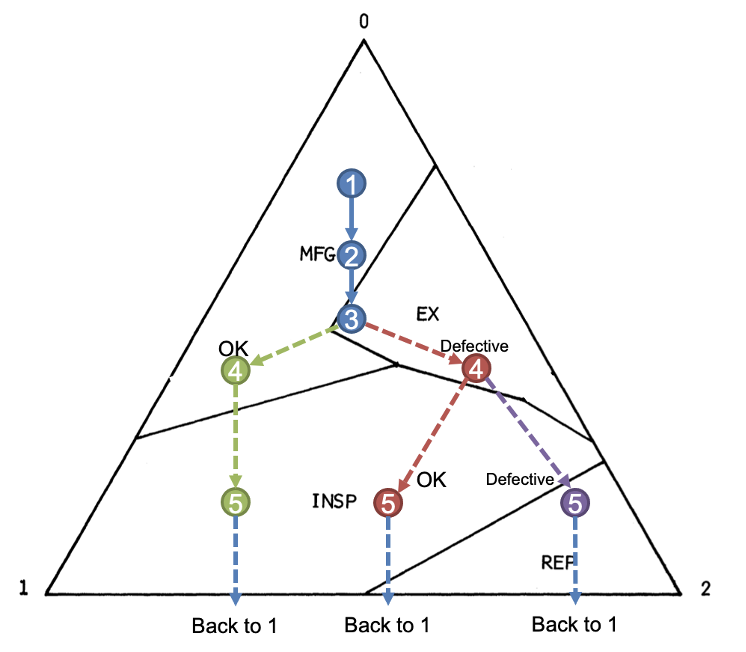
\includegraphics[width=8cm]{smith_1.png}
\end{center}
\end{question}

\begin{answer} 
    \\
    \begin{center}
        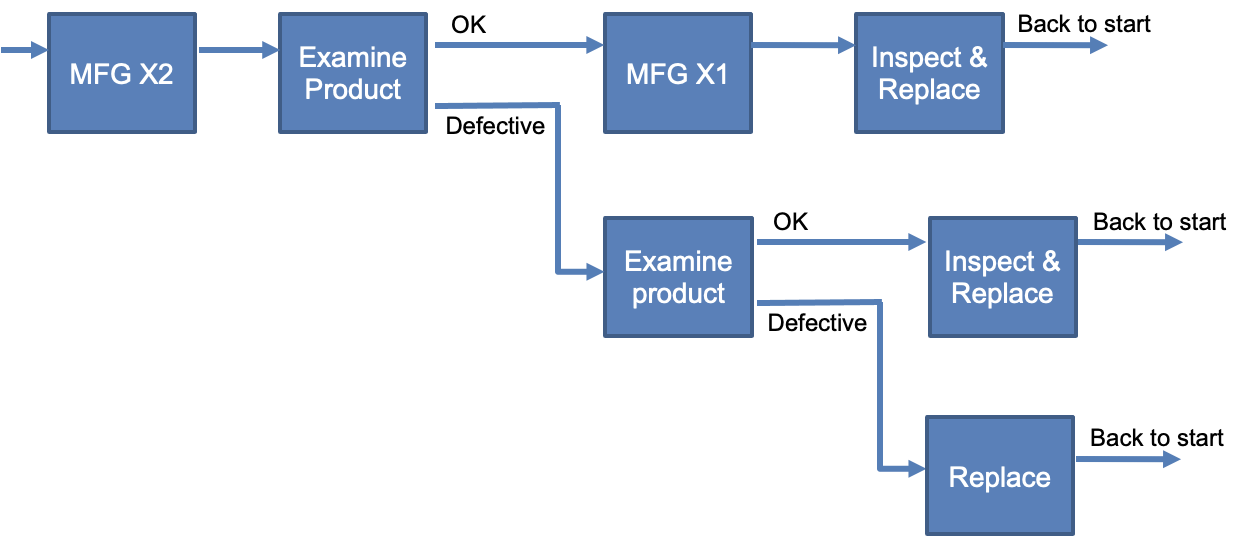
\includegraphics[width=10cm]{smith_2.png}
    \end{center}
\end{answer}

\begin{question}
    Define the complexity classes P, NP, PSPCAE, and NC. What does it mean for a problem A to be INSERT COMPLEXITY CLASS-complete?
\end{question}

\begin{answer}
    \begin{enumerate}
        \item P = decidable in polynomial time
        \item NP = decidable in nondeterministic polynomial time
        \item PSPACE = decidable in polynomial space
        \item NC = decidable in polylogarithmic time on a parallel machine
    \end{enumerate}
\end{answer}

\begin{question}
If A is in class X and can be reduced to some other X-complete problem we say A is X-complete. This means A is of complexity class X and at least as hard as every other problem in class X
Sketch the reduction showing deterministic MDPs are in complexity class NC (parallelizable)
\end{question}

\begin{answer}
    \begin{enumerate}
        \item Let M be a deterministic MDP with states $s_i \in S$ and state transition probability p of 0 or 1 and goal to minimize cost c
        \item Reduction to shortest path:
            \begin{enumerate}
                \item Let $G=(V,E)$ be a graph
                \item Let $v_i$ connect to $v_j$ by edge $e_{i,j}$ of cost $c_{s_i,s_j}$ iff there is a MDP transition from state $s_i$ to $s_j$ 
                \item Let $v_0$ equate to initial state $s_0$ 
            \end{enumerate}
        \item Finding the shortest path from $v_0$ to some final node $v_T$ is equivalent to minimizing the MDP with initial state $s_0$ and final state $s_T$
        \item We know that finding the shortest path in a graph $G$ is computable in NC, thus the reduction is complete
    \end{enumerate}
\end{answer}

\begin{question}
    The resampling step in a standard bootstrap filter algorithm is given as:

\begin{align}
    \text{ For } i = 1, \cdots, N, \text{ sample } x_t^{(i)} \sim \tilde{\pi}_{t|t}^N(dx_t).
\end{align}

What is the purpose of this resampling step?
\end{question}

\begin{answer}
    In the sampling step, one obtains a set of particles $\{\tilde{x}_t^{(i)}\}^N_{i=1}$ whose "unweighted" empricial distribution $\tilde{\pi}_{t|t}^N(dx_t)$ is an Monte Carlo approximation of $\pi_{t|t-1}(dx_t)$. The weighted empriical distribution $\tilde{\pi}_{t|t}^{N}(dx_t)$ approximates $\pi_{t|t}(dx_t)$. The aim of the resampling step is to obtain an unweighted empirical distribution approximation $\pi_{t|t}^N(dx_t)$ of $\tilde{x}_{t|t}^N(dx_t)$ by duplicating particles having high weights and discarding others to focus on the zones of high posterior probabilities.
\end{answer}

\begin{question}
    Under what cases/assumptions is simple convergence and/or uniform convergence of the mean squared error towards zero guaranteed for a particle filter?  What is the rate of convergence? Does the particle filter beat the curse of dimensionality?
\end{question}

\begin{answer}
    We first assume that the transition kernel $K$ is Feller and that the likelihood function $g$ is bounded, continuous, and strictly positive.

If the importance weights are upper bounded, and one uses a standard resampling scheme, simple convergence of the mean squared error towards zero is ensured, with rate of convergence of $1/N$. If the transition kernel is weakly dependent on the past value, i.e. if the "true" optimal filter is quickly mixing, then uniform convergence of the particle filter is ensured, with rate of convergence of $1/N$.

Although the rate of convergence does not depend on the state dimension, for simple convergence, to ensure a given precision on the mean squared error, the number of particles N depends on $c_{t|t}$ which is dependent on $n_x$. Therefore, particle filters under simple convergence does not beat the curse of dimensionality. Under uniform convergence, particle filters do indeed beat the curse of dimensionality, as ensuring a given precision on the mean squared error also does not depend on $n_x$.
\end{answer}

\begin{question}
    Given the algorithm presented by the researchers for sparse sampling, what
is the minimum sufficient depth and width necessary to guarantee a value
function approximate accuracy within 0.01 for an MDP defined by:

$$Rmax = 100$$
$$\gamma = 0.95$$
$$|A| = 2$$
\end{question}

\begin{answer}
$$H = 382$$
$$C \approx 3.5852849668449816e21$$
\end{answer}

\begin{question}
    What is the running time lower bound for any planning algorithm with access only to a generative model?  Why is it this value?
\end{question}

\begin{answer}
    The running time lower bound is proven by the trivial example of a binary tree with depth H.
An MDP defined by 2 actions and deterministic transition probabilities is described completely
by this tree. In order to find the near optimal policy, an algorithm A must search this tree
and find the rewarding node v given initial state s0. At least $\Omega(2^H)$ calls to the generative
model must be made in this case (same as with other tree search methods).
\end{answer}

\section{Questions from Lectures}

\begin{question}
    Give an asymptotic upper bound (using Big-O notation) of the running time of value iteration applied to a discrete MDP with fixed horizon $H$ with respect to the horizon and the sizes of the state and action spaces.
\end{question}

\begin{answer}
    The value iteration algorithm can be expressed as
    \begin{algorithmic}[1]
        \For{$t \in \{H, H-1, \ldots, \}$}
            \For{$s \in \mathcal{S}$}
            \State $V_t(s) = \max_{a \in \mathcal{A}}\left(R(s, a) + \gamma \sum_{s'\in\mathcal{S}} T(s'\mid s, a) V_{t+1}(s')\right)$ \label{ln:bellman}
            \EndFor
        \EndFor
    \end{algorithmic}
    Line~\ref{ln:bellman} is executed $|\mathcal{S}| H$ times.
    The maximization in line 3 can be accomplished by looping over all of the actions, which requires $|\mathcal{A}|$ executions of $R(s, a) + \gamma \sum_{s'\in\mathcal{S}} T(s'\mid s, a) V_{t+1}(s')$. 
    The sum requires $O(|\mathcal{S}|)$ operations. Thus the running time is $O(H|\mathcal{A}||S|^2)$.
\end{answer}

\begin{question}
    Indicate whether the following statements are true, false, or unknown:
    \begin{enumerate}[label=\alph*)]
        \item P $\subsetneq$ NP
        \item NP $\subseteq$ PSPACE
        \item A PSPACE-hard problem must by definition be in PSPACE
        \item A PSPACE-complete problem must by definition be in PSPACE
        \item There are algorithms that run in exponential time that can solve problems in P
        \item Every abstract problem in PSPACE requires an exponential-time algorithm to solve it
    \end{enumerate}
\end{question}

\begin{answer} 
     \begin{enumerate}[label=\alph*)]
        \item unknown
        \item true
        \item false
        \item true
        \item true
        \item false
    \end{enumerate}
\end{answer}

\begin{question}
    Use an example to explain why almost sure, rather than sure convergence is used more often in mathematical literature involving random variables.
\end{question}

\begin{answer}
    In the case of Monte Carlo integration, there is an $\omega \in \Omega$ for which the same point is sampled over and over again, so it is impossible to prove sure convergence.
\end{answer}

\begin{question}
    Let $Y$ be a random variable that takes values in [-1, 1] with mean -0.5. Give an upper bound on the probability that $Y \geq 0.5$.
\end{question}

\begin{answer}
    Let $Z=Y+1$, then $P(Z \geq 1.5) = P(Y \geq 0.5)$ and $Z$ is positive, so we can use Markov's inequality:
    $$P(Z \geq 1.5) \geq \frac{E[Z]}{1.5} = \frac{0.5}{1.5} = \frac{1}{3}$$
    so the probability is less than $\frac{1}{3}$.
\end{answer}

\end{document}
